
\chapter{Lehrplanung (Unterrichte)}
\label{chap:lessons}

Die Lehrplanung wird in Untis mit der Ressource Unterrichte modelliert, welche sich aus den Ressourcen der Stammdaten zusammensetzt. Sie sind die Instanzen eines Faches, gehalten in einer Unterrichtsform von einem Dozenten in einem Raum, für bestimmte Studentengruppen.\\
\\
Unterricht erreicht man in dem man die Pfeile unter die vier Hauptstammdaten betätigt und \texttt{Unterrichte} anklickt.

\begin{figure}[h]
	\centering
	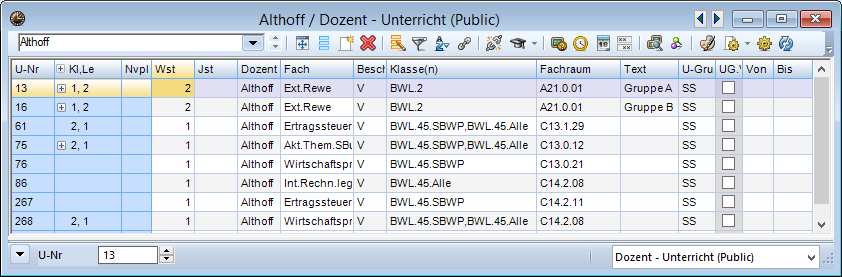
\includegraphics[width=.8\textwidth]{unterrichte}
	\vspace{-5pt}
	\caption{Unterrichte}
	\label{fig:unterrichte}
\end{figure}

\section{Attribute}

\noindent
\texttt{U-Nr} (Schlüssel-Wert):  Die von Untis gegebene Schlüssel-Wert. Unterrichte können keine eindeutigen Namen halten, daher assoziiert Untis sie mit Nummern. Diese werden für viele Meldungen verwendet.  (Nicht Editierbar)\\

\noindent
\texttt{Kl,Le} (Anzahl Gruppen, Dozenten):  Die Anzahl der, mit dem Unterricht assoziierte, Gruppen und Dozenten. Die Werte an sich werden für nichts verwendet. Das kleine Plus-Zeichen wird für die Inline-Bearbeitung der Kopplungszeilen benutzt. (Nicht Editierbar)\\

\noindent
\texttt{Nvpl}:  Die Anzahl der nicht verplante Stunden. (Nicht Editierbar)\\

\noindent
\texttt{Wst} (Reguläre Stunden):  Die Anzahl der regulären Stunden pro Woche für diesen Unterricht. (Pflicht bei reguläre Veranstaltungen, sehe \secref{sec:zeitverlauf})\\

\noindent
\texttt{Jst} (Sporadische Stunden):  Die Anzahl der sporadischen, über das Jahr verteilte Stunden, in dem Stunden für diesen Unterricht stattfinden sollte. (Pflicht bei sporadische Veranstaltungen, sehe \secref{sec:zeitverlauf})\\

\noindent
\texttt{Dozent}:  Der Dozent, der diese Veranstaltung hält. Um mehrere Dozenten einem Unterricht zuzuweisen, werden Kopplungszeilen benötigt, sehe \secref{sec:kopplungszeilen}. (Pflicht)\\

\noindent
\texttt{Fach}:  Das Fach des Unterrichts. Um mehrere Fächer einen Unterricht zuzuweisen, werden Kopplungszeilen benötigt, sehe \secref{sec:kopplungszeilen}. (Pflicht)\\

\noindent
\texttt{Beschr.} (Unterrichtsmethode):  Die Methode bzw. Methoden des Unterrichts. (Pflicht)\\

\noindent
\texttt{Klasse(n)} (Gruppen):  Studierenden, die diesen Unterricht besuchen sollten, oder die Gruppe von Fächer, zu dem dieser Unterricht gehört. Mehrere Gruppen müssen Komma-getrennt hintereinander aufgelistet werden. (Pflicht)\\

\noindent
\texttt{Fachraum}:  Der angedachte Raum oder Raumgruppe, die bei der Planung verwendet werden sollte. (Optional, Zuordnung muss spätestens bei der Stundenplanung eingetragen werden.)\\

\noindent
\texttt{Text} (Kommentar):  Ein Kommentar der zusätzliche Informationen zum Unterricht liefert, z.B ``Gruppe C", \hspace{1pt} ``14-täglich" \hspace{1pt} oder ``ab 14 Uhr" \hspace{1pt}. Sollten Sie Untis zur Stundenplan-Darstellung verwenden es wird empfohlen dieses Feld mit einem ``." \hspace{1pt} wegen ein Bug in Untis zu belegen. Siehe \secref{sec:stundenplan-stunde}. (Optional)\\

\noindent
\texttt{U-Gruppe} (Verlauf):  Der Zeitverlauf des Unterrichts. (Pflicht bei reguläre Veranstaltungen, Empfohlen bei sporadische Veranstaltungen)\\

\noindent
\texttt{Von} (Startdatum):  Das einschließliche Startdatum, sehe \secref{sec:zeitverlauf}. (Situationsabhängig)\\

\noindent
\texttt{Bis} (Enddatum):  Das einschließliche Enddatum, sehe \secref{sec:zeitverlauf}. (Situationsabhängig)\\

\section{Kopplungszeilen}
\label{sec:kopplungszeilen}

Sollte mehrere Dozenten oder mehrere Fächer zu einem Unterricht untergeordnet, werden auch mehrere Zeilen nötig (genau: Anzahl Dozenten * Anzahl Fächer). Es gibt zwei Methoden, um Kopplungszeilen zu erzeugen, ``Inline-Bearbeitung" \hspace{1pt} und die \texttt{Koppeln}-Ansicht.

\newpage

\begin{figure}[h]
	\centering
	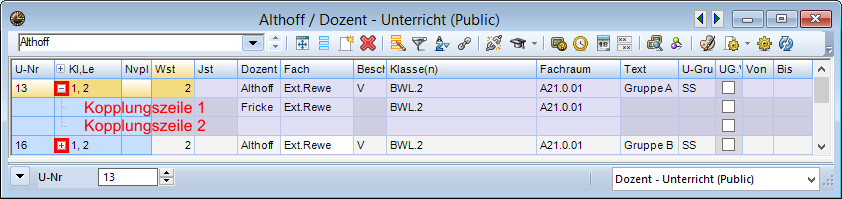
\includegraphics[width=.8\textwidth]{kopplungszeilen}
	\vspace{-5pt}
	\caption{Kopplungszeilen}
	\label{fig:kopplungszeilen}
\end{figure}

\subsection{Inline-Bearbeitung}

Durch die Inline-Bearbeitung gelangt man zu der Darstellung, in der man die Zeilen untereinander schreibt. Die zweite Zeile öffnet sich, indem man mit der Maus über die Spalte \texttt{Kl,Le} bringt und und dort das erscheinende $+$ Symbol anklickt.\\
\\
Diese lässt die erste Kopplungszeile erscheinen. Sofern Daten in einer Zeile eingetragen sind, erscheint eine Zeile für weitere Einträge. In den neuen Zeilen sind einige Felder nicht editierbar: Stundenangaben, Unterrichtsmethode, Kommentar und der Verlauf. Die Angaben der Hauptzeile gelten für alle Kopplungszeilen. Hier muss man sich auf die zusätzliche Dozenten oder Fächer beschränken, dennoch wird empfohlen, alle Kopplungszeilen so vollständig wie möglich auszufüllen.

\subsection{Koppeln-Ansicht}

\begin{wrapfigure}{r}{0.35\textwidth}
	\vspace{-14pt}
	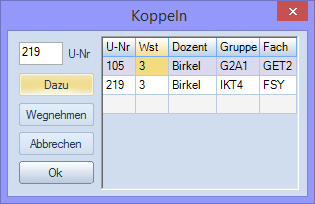
\includegraphics[width=.34\textwidth]{koppeln-ansicht}
	\vspace{-5pt}
	\caption{Koppeln-Ansicht}
	\label{fig:koppeln-ansicht}
\end{wrapfigure}

Die \texttt{Koppeln}-Ansicht bietet die Möglichkeit, unabhängige Unterrichte zusammenzufassen. Dazu klickt man auf eine Zeile, dann das \texttt{Koppeln} Symbol. Die Ansicht öffnet sich mit dem, in der Auflistung der Unterrichte, markierte Unterricht bereits eingetragen. Um weitere hinzuzufügen, trägt man im Feld \texttt{U-Nr} die Nummer eines Unterrichts die an dieser gekoppelt werden sollten ein, der an diesen gekoppelt werden soll und drückt auf \texttt{Dazu}. Die Vorauswahl von mehrere vom Stundenplan-Ansicht funktioniert nicht. Um eine Zeile zu entfernen, klickt man entsprechend auf \texttt{Wegnehmen}. Um die Änderungen wirksam zu machen, klickt man anschließend auf \texttt{Ok}. Um die Änderungen zu verwerfen, drückt man \texttt{Abbrechen}, oder schließt das Fenster.

\newpage

\subsection{Entkoppeln-Ansicht}

Das Entkoppeln von Zeilen erfolgt allein über die Entkoppeln-Ansicht. Dieser macht aus einzelne Zeilen eigenständige Unterrichte. Man gelangt zu dieser Ansicht, indem man auf das \texttt{Erweitertes Entkoppeln} Symbol klickt. Um Zeilen einzeln eigenständig zu machen, klickt man auf die Zeile, gefolgt vom $\Leftrightarrow$ Symbol. Man kann auch alle Zeilen eigenständig machen, in dem man auf \texttt{Alle Entkoppeln} drückt. Letzteres ist unter Umständen gefährlich, denn die Änderungen werden sofort wirksam und der Ansicht schließt sich. Um die Änderungen sonst anzunehmen, klickt man anschließend auf \texttt{Ok}. Um die Änderungen zu verwerfen, drückt man \texttt{Abbrechen}, oder schließt das Fenster.

\begin{figure}[h]
	\centering
	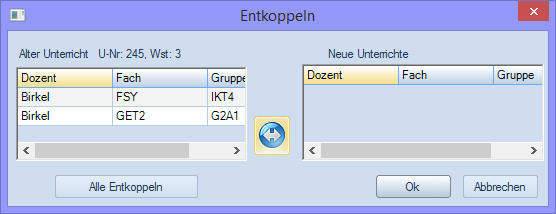
\includegraphics[width=.6\textwidth]{entkoppeln-ansicht}
	\vspace{-5pt}
	\caption{Entkoppeln-Ansicht}
	\label{fig:entkoppeln-ansicht}
\end{figure}


\section{Zeitverlauf}
\label{sec:zeitverlauf}

Der Zeitverlauf bezieht sich auf die Stundenangaben, Unterrichtsgruppe und ggf. Start-/Enddatum. Dementsprechend wird hier vertiefend auf Unterrichtsgruppen und ihren Bezug zum Unterricht eingehen.

\subsection{Verläufe (Unterrichtsgruppen)}

Verläufe, \texttt{Unterrichtsgruppen}, wie in \secref{sec:unterrichtsgruppen}, beschrieben, regeln die Termine an denen ein Unterricht stattfinden darf. Deshalb ist diese Angabe, außer bei Unterrichten, die gänzlich von Anderen abweichen, angebracht. Hierdurch kann man Aussagen machen wie der Unterricht geschieht in den regulären Vorlesungszeiten, in der B-Woche, in der Projektwoche, oder in einer bestimmten Klausurwoche.

\subsection{Start- \& Enddaten (Von  \& Bis)}

Zusätzlich kann man den allein oder im Zusammenspiel mit Unterrichtsgruppen Start-, \texttt{Von}, und/oder Enddaten, \texttt{Bis}, angeben. Wenn z.B., ein Unterricht in der regulären Vorlesungszeit stattfindet und wird nicht durch die Projektwochen unterbrochen, könnte man genauso gut nur der Start- und Enddatum der regulären Vorlesungszeit bei der Unterricht eintragen. Im Zusammenspiel kann man Aussagen machen wie der er findet in der reguläre Vorlesungszeit ab, bzw. bis, einem Datum, oder dass eine Veranstaltung nur in der zweite Woche einer der Blockzeiten gehalten wird.

\subsection{Reguläre Stunden (Wochenstunden)}

Reguläre Stunden, \texttt{Wochenstunden}, sagen einen wie viele Blöcke ein Unterricht in einer Woche gehalten wird. Ohne Unterrichtsgruppe, Start- oder Enddatum gilt der Unterricht für die gesamte sechs Monaten die zu einem Semester gehören. Im Zusammenspiel mit einer Unterrichtsgruppe kann man aussagen machen wie der Unterricht findet zwei mal der Woche jeder A-Woche der reguläre Vorlesungszeit, oder dass ein Unterricht 30 mal die Woche im zweiten zweiwöchigen Blockzeit des Wintersemesters. Auch hier können Start- und Enddaten benutzt werden um noch kompliziertere Aussagen über den Verlauf zu machen.

\subsection{Sporadische Stunden (Jahresstunden)}

Zum Schluss gibt es auch noch sporadische Stunden, \texttt{Jahresstunden}. Diese verwendet man um Unterrichte darzustellen die, theoretisch, über das gesamte Jahr stattfinden können. Um diese zu gewährleisten verlangt Untis, dass alle Ressourcen die mit einem solchen Unterricht assoziiert werden auch in allen Perioden vorhanden sind und wird eine Fehlermeldung geben sobald sporadische Stunden im Zusammenhang mit eine solche Ressource verbunden werden sollte.\\
\\
Praktisch gesehen ist dies nie der Fall deswegen empfehle ich, sofern möglich, sporadische Stunden nicht zu verwenden. Doch bei Ausfälle machen sich Jahresstunden recht nützlich. Angenommen ein Unterricht mit regulären Stunden soll an einem bestimmten Datum ausfallen. Man trägt in der Jahresstunden Attribute zum Unterricht das Zeichen ``*" \hspace{1pt} ein. Diese wandelt vorhandene geplante reguläre Stunden in sporadische um. Zum Beispiel, war eine Veranstaltung an 13 Wochen für zwei Blöcke geplant, werden nach der Umwandlung 26 Jahresstunden eingetragen sein. Dieser Kniff wird später nochmals verdeutlicht in \secref{sec:manuelle-entplanung}.



















